\documentclass[a4paper]{article}

\usepackage[a4paper,top=2cm,bottom=2cm,left=3cm,right=3cm,marginparwidth=1.75cm]{geometry}
\usepackage[utf8]{inputenc}
\usepackage[T1]{fontenc}
\usepackage{textcomp}
\usepackage[ngerman]{babel}
\usepackage{amsmath, amssymb, nccmath}
\usepackage{accents}


\usepackage{multirow}
\usepackage{fancyhdr}
\usepackage{lastpage}

% figure support
\usepackage{import}
\usepackage{xifthen}
\pdfminorversion=7
\usepackage{pdfpages}
\usepackage{transparent}
\newcommand{\incfig}[1]{%
    \def\svgwidth{\columnwidth}
    \import{./figures/}{#1.pdf_tex}
}

\pdfsuppresswarningpagegroup=1

\title{Protokoll zur sechsten Laborübung\\Messtechnik Labor 376.091}
\author{DINC Atilla (11917652)}

\begin{document}
\newcommand{\unit}[1]{\ensuremath{\, \mathrm{#1}}} % Einheiten in Math-Moder richtig formatieren
% --------------------- HEADER ---------------------
\pagestyle{fancy}
% --------------------- FOOTER ---------------------
\fancyfoot[L]{Wintersemester 2023}
\fancyfoot[C]{\textbf{\thepage /\pageref{LastPage}}}
\renewcommand{\footrulewidth}{0.4pt}

\normalsize
\maketitle
\tableofcontents
\pagebreak
\section{Erklärung, Unterschrift, Allgemeines}
Alle Messungen und Ergebnisse die diesem Protokoll entstammen wurden von Atilla Dinc,
Muhammend Tesgin und Victoria Wolfgruber durchgeführt und dokumentiert.

\begin{figure}[h]
    \centering
    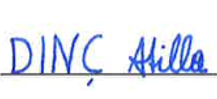
\includegraphics[width=0.3\textwidth]{images/Unterschrift}
    \caption{Unterschrift des Protokollführers DINC Atilla}
\end{figure}

\subsection{Teilnehmerinformationen}
	\begin{tabular}{|c| c|}
		\hline
        \textbf{Gruppennummer:} & 5                                                                                        \\
        \hline
		\multicolumn{2}{|c|}{\textbf{Gruppenmitglider}}                                                                                        \\
		\hline
        Name & Matrikelnummer\\
        \hline
        Atilla Dinc & 11917652\\
        Muhammed Tesgin & 12004145\\
        Victoria Wolfgruber & 11933423\\
        \hline
	\end{tabular}

\subsection{Laborausstattung}
\begin{center}
	\begin{tabular}{|c| c| c| c| c|}
		\hline
		\multicolumn{5}{|c|}{\textbf{Geräteliste}}                                                                                        \\
		\hline

		Bezeichnung              & Gerätebeschreibung                                         & Messgrößen & Inventarnummer & Bemerkungen \\
		\hline
		OZ1                      & ADigitalspeicheroszilloskop DSO-x2002A                                  & -          & CD0408-7         & -           \\
		MM1                       & Digitalmultimeter                                          & -          & CA0402-1            & -           \\
		DAQ                      & CaptureCard                      & -   & CA0410-3       & -           \\
		DAC                      & DAQ-Anschluss                       & -   & CA0410-3       & -           \\
		                         & Reflektor                                          & -    & CA0410-2        & -           \\
		\hline
		\hline
		\multicolumn{5}{|c|}{\textbf{Zubehörliste}}                                                                                       \\
		\hline
		Bezeichnung              & Zubehörbeschreibung                                        & Messgrößen & Inventarnummer & Bemerkungen \\
		\hline
		RF1                       & Reflektoraufsatz & -          & -              &     -    \\
		RF2                       & Reflektoraufsatz & -          & -              &     -    \\
		\hline
	\end{tabular}
\end{center}

% ~~~~~~~~~~~~~~~~~~~~~~~~~~~~ Start of the document ~~~~~~~~~~~~~~~~~~~~~~~~~~~~

\newpage
\section{Einleitung}
In dieser Laborübung soll der Umgang mit den gängigen Messgeräten geübt werden.
Weiters soll ein intuitives Verständnis für die grundlegenden Funktionen,
Einschränkungen und Fehlerquellen geschult werden.\newline 


\end{document}
